
\documentclass[letterpaper, reqno,11pt]{article}
\usepackage[margin=1.0in]{geometry}
\usepackage{color,latexsym,amsmath,amssymb}
\usepackage{fancyhdr}
\usepackage{amsthm}
\usepackage[linesnumbered,lined,boxed,commentsnumbered,noend,noline]{algorithm2e}
\usepackage{dsfont}
\usepackage{graphicx}
\usepackage{hyperref}
\usepackage{bbm}
\usepackage[inline]{enumitem}
\usepackage[numbers]{natbib}
\usepackage{framed}
\usepackage{titling}
\usepackage{subcaption}
\usepackage[dvipsnames]{xcolor}
\usepackage{tikz}

\tikzset{invclip/.style={clip,insert path={{[reset cm]
  (-16383.99999pt,-16383.99999pt) rectangle (16383.99999pt,16383.99999pt)}}}}

\allowdisplaybreaks

\newcommand{\RR}{\mathbb{R}}
\newcommand{\CC}{\mathbb{C}}
\newcommand{\ZZ}{\mathbb{Z}}
\newcommand{\QQ}{\mathbb{Q}}
\newcommand{\NN}{\mathbb{N}}
\newcommand{\FF}{\mathbb{F}}
\newcommand{\PP}{\mathbb{P}}
\newcommand{\EE}{\mathbb{E}}
\newcommand{\LL}{\mathbb{L}}
\newcommand{\TT}{\mathbb{T}}
\DeclareMathOperator{\conv}{conv}
\DeclareMathOperator{\charcone}{char.cone}
\DeclareMathOperator{\STAB}{STAB}
\DeclareMathOperator{\Down}{Down}
\DeclareMathOperator{\lca}{lca}
\DeclareMathOperator{\ex}{ex}
\DeclareMathOperator{\Span}{span}
\DeclareMathOperator{\T}{T}
\DeclareMathOperator{\F}{F}
\DeclareMathOperator{\shP}{\# P}
\DeclareMathOperator{\shSAT}{\# SAT}
\DeclareMathOperator{\shDNF}{\# DNF}
\DeclareMathOperator{\DNF}{DNF}
\DeclareMathOperator{\Poly}{P}
\DeclareMathOperator{\CNF}{CNF}
\DeclareMathOperator{\SAT}{SAT}
\DeclareMathOperator{\BPP}{BPP}
\DeclareMathOperator{\poly}{poly}
\DeclareMathOperator{\sign}{sign}
\newcommand\mycommfont[1]{\ttfamily\textcolor{blue}{#1}}
\SetCommentSty{mycommfont}
\begin{document}
\pagenumbering{arabic}
\title{Lectures on Polynomial Identity Testing}
\author{Yuchong Pan}
\date{\today}
\newtheorem{theorem}{Theorem}
\newtheorem{lemma}[theorem]{Lemma}
\newtheorem{proposition}[theorem]{Proposition}
\newtheorem{corollary}[theorem]{Corollary}
\newtheorem{fact}[theorem]{Fact}
\newtheorem{problem}[theorem]{Problem}
\newtheorem{claim}{Claim}
\newtheorem{exercise}{Exercise}
\theoremstyle{definition}
\newtheorem{definition}[theorem]{Definition}
%\maketitle
%

\begin{framed}
\noindent{\bf 6.842 Randomness and Computation} \hfill \thedate
\begin{center}
\Large{\thetitle}
\end{center}
\noindent{\em Lecturer: Ronitt Rubinfield} \hfill {\em Scribe: \theauthor}
\end{framed}

\section{Univariate Polynomial Identity Testing}

Polynomial identity testing asks whether two polynomials are identical, e.g., $P(x) = (x + 3)^{38} (x - 4)^{83}$ and $Q(x) = (x - 4)^{38} (x + 3)^{83}$? The following two problems are equivalent:

\begin{problem}
  Given two polynomials $P, Q$ of degree at most $d$, is $P \equiv Q$?
\end{problem}

\begin{problem}
  Given two polynomials $P$ of degree at most $d$, is $P \equiv 0$?
\end{problem}

Recall the following fundamental fact of algebra:

\begin{fact} \label{fact:poly}
  If $R$ is a polynomial of degree at most $d$ with $R \not \equiv 0$, then $R$ has at most $d$ roots.
\end{fact}

Fact \ref{fact:poly} implies a simple algorithm to test if a polynomial is identical to $0$, given in Algorithm \ref{alg:simple}. This algorithm requires $O(d)$ evaluations of $R$.

\begin{algorithm}
  pick $d + 1$ points $x_1, \ldots, x_{d + 1}$ \\
  \If{$R(x_i) = 0 \;\forall i \in [d + 1]$}{
    output ``$R \equiv 0$''
  }
  \Else{
    \CommentSty{// $\exists i \in [d + 1] \text{ s.t.\ } R(x_i) \neq 0$} \\
    output ``$R \not \equiv 0$''
  }
  \caption{A simple algorithm for testing whether a polynomial $R$ of degree at most $d$ is identical to $0$.}
  \label{alg:simple}
\end{algorithm}

Indeed, we can design a faster randomized algorithm to test if a polynomial is identical to $0$, given in Algorithm \ref{alg:rand}. If $R \equiv 0$, the algorithm will always output ``$R \equiv 0$.'' If $R \not \equiv 0$, in each loop,
$$ \PP_{i \in [2d]}\left[R\left(x_i\right) = 0\right] \leq \frac{\text{\# roots}}{2d} \leq \frac{d}{2d} = \frac{1}{2}. $$
Therefore,
$$ \PP[\text{error}] = \PP[\text{choose roots in all $k$ iterations}] \leq \frac{1}{2^k}. $$
It follows that
$$ \PP[\text{output ``$R \not \equiv 0$''}] \geq 1 - \frac{1}{2^k}. $$
If we tolerate the probability of error to be at most $\delta$, then we pick $k = \log 1/\delta$ (which does not depend on $d$), and the probability of outputting ``$R \not \equiv 0$'' is at least $1 - \delta$.

\begin{algorithm}
  \SetKwFor{RepTimes}{repeat}{times}{end}
  pick $2d$ distinct points $x_1, \ldots, x_{2d}$ \\
  \RepTimes{$k$}{
    pick $i \in [2d]$ \\
    \If{$R(x_i) \neq 0$}{
      output ``$R \neq 0$'' \\
      \Return
    }
  }
  output ``$R \equiv 0$''
  \caption{A faster randomized algorithm for testing whether a polynomial $R$ if degree at most $d$ is identical to $0$.}
  \label{alg:rand}
\end{algorithm}

\subsection{Application: Person on the Moon}

The ``person on the moon'' problem is formulated as follows: A person on the earth has an $(n + 1)$-bit string $w = w_0 \ldots w_n$. A person on the moon has another $(n + 1)$-bit string $w^* = w_0^* \ldots w_n^*$. The question is whether $w = w^*$.

Let
\begin{align*}
  P(x) &= w_n x^n + w_{n - 1} x^{n - 1} + \ldots + w_1 x + w_0, \\
  P^*(x) &= w_n^* x^n + w_{n - 1}^* x^{n - 1} + \ldots + w_1^* x + w_0^*.
\end{align*}
Then $P$ and $P^*$ are polynomials of degree $n$. Moreover, $w = w^*$ if and only if $P \equiv P^*$. Here is the general strategy motivated by polynomial identity testing:
\begin{itemize}[itemsep=0pt]
  \item The earth person picks random $r_1, \ldots, r_k$ and sends
  \begin{gather*}
    \left(r_1, P\left(r_1\right)\right), \qquad \left(r_2, P\left(r_2\right)\right), \qquad \ldots, \qquad \left(r_k, P\left(r_k\right)\right).
  \end{gather*}
  \item The moon person checks equality on $r_1, \ldots, r_k$.
\end{itemize}
Each $r_i$ for $i \in [k]$ requires $\Theta(\log n)$ bits of communication. However, a polynomial of degree $n$ evaluated on an input of $\Theta(\log n)$ bits can give values as large as $\Theta(n^n)$ (which rquires $\Theta(n \log n)$ bits to describe). To fix this issue, we can use a prime $q$ of $O(\log n)$ bits and send every number modulo $q$. Therefore, the total number of bits is $O(k \log n)$.

\section{Multivariate Polynomial Identity Testing}

In this section, we study multivariate polynomial identity testing:

\begin{problem}
  Given a multivariate polynomial $R$ on $n$ variables $x_1, \ldots, x_n$, is $R \equiv 0$?
\end{problem}

\begin{definition}
  Given a multivariate polynomial $R$ on $n$ variables $x_1, \ldots, x_n$, the \emph{total degree} of $R$ is defined to be
  $$ \max_{s: \text{ term of $R$}} (\text{sum of degrees of the $x_i$'s in $s$}). $$
\end{definition}

Multivariate polynomial identity testing have the following two difficulties:
\begin{itemize}[itemsep=0pt]
  \item \emph{Difficulty 1:} A multivariate polynomial $R \not\equiv 0$ can have infinitely many roots, e.g., $R(x, y) = x \cdot y$ and $R(x, y) = x - y$.
  \item \emph{Difficulty 2:} The number of terms in a multivariate polynomial of total degree $d$ can be $\binom{n}{d}$.
\end{itemize}

\begin{theorem}[Schwartz-Zippel-De Mill Lipton]
  Let $R$ be a multivariate polynomial of degree $d$ on $n$ variables $x_1, \ldots, x_n$ such that $R \not \equiv 0$. Let $S$ be a set of points such that $|S| = 2d$. Pick $x_i \in_R$ for all $i \in [n]$. Then
  $$ \PP\left[R\left(x_1, \ldots, x_n\right) = 0\right] \leq \frac{d}{|S|}. $$
\end{theorem}

\subsection{Application: Bipartite Perfect Matching}

\begin{definition}
  Let $G = (A \sqcup B, E)$ be a bipartite graph. A \emph{matching} is a subset $M \subseteq E$ in which no two edges share a vertex. A \emph{perfect matching} is a matching $M$ such that $|V[M]| = n$.
\end{definition}

\begin{definition}
  Let $G = (A \sqcup B, E)$ be a bipartite graph. Let $x_{u, v}$ be a variable for each $u \in A, v \in B$. The \emph{Tutte matrix} of $G$ is defined to be an $|A| \times |B|$ symbolic matrix $A = (a_{u, v})_{u \in A, v \in B}$ such that
  $$ a_{u, v} = \left\{
    \begin{array}{ll}
      x_{u, v}, & \text{if $(u, v) \in E$}, \\
      0, & \text{otherwise}.
    \end{array}
  \right. $$
\end{definition}

\noindent\emph{Example.} Let $G$ be the graph in Figure \ref{subfig:graph}. Figures \ref{subfig:pm1} and \ref{subfig:pm2} give two perfect matchings in $G$. Moreover, the Tutte matrix $A_G$ of $G$ is given by
$$ A_G = \begin{pmatrix}
  x_{1, a} & x_{1, b} & 0 \\
  x_{2, a} & x_{2, b} & 0 \\
  x_{3, a} & 0 & x_{3, c}
\end{pmatrix}, $$
where the rows are indexed by the vertices on the left side, and the columns are indexed by the vertices on the right side. We have
$$ \det A_G = x_{1, a} x_{2, b} x_{3, c} - x_{1, b} x_{2, a} x_{3, c}. $$

\begin{figure}[h]
  \centering
  \begin{subfigure}[c]{.32\textwidth}
    \centering
    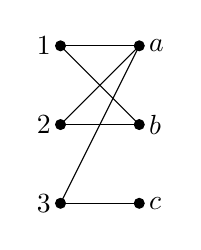
\begin{tikzpicture}
      \fill[black] (0, 0) circle (2pt) node[left] {$1$};
      \fill[black] (0, -1) circle (2pt) node[left] {$2$};
      \fill[black] (0, -2) circle (2pt) node[left] {$3$};
      \fill[black] (1, 0) circle (2pt) node[right] {$a$};
      \fill[black] (1, -1) circle (2pt) node[right] {$b$};
      \fill[black] (1, -2) circle (2pt) node[right] {$c$};
      \draw (0, 0) -- (1, 0);
      \draw (0, 0) -- (1, -1);
      \draw (0, -1) -- (1, 0);
      \draw (0, -1) -- (1, -1);
      \draw (0, -2) -- (1, 0);
      \draw (0, -2) -- (1, -2);
    \end{tikzpicture}
    \caption{The graph $G$.}
    \label{subfig:graph}
  \end{subfigure}
  \hfill
  \begin{subfigure}[c]{.32\textwidth}
    \centering
    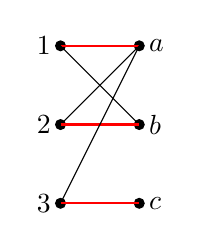
\begin{tikzpicture}
      \fill[black] (0, 0) circle (2pt) node[left] {$1$};
      \fill[black] (0, -1) circle (2pt) node[left] {$2$};
      \fill[black] (0, -2) circle (2pt) node[left] {$3$};
      \fill[black] (1, 0) circle (2pt) node[right] {$a$};
      \fill[black] (1, -1) circle (2pt) node[right] {$b$};
      \fill[black] (1, -2) circle (2pt) node[right] {$c$};
      \draw[red, thick] (0, 0) -- (1, 0);
      \draw (0, 0) -- (1, -1);
      \draw (0, -1) -- (1, 0);
      \draw[red, thick] (0, -1) -- (1, -1);
      \draw (0, -2) -- (1, 0);
      \draw[red, thick] (0, -2) -- (1, -2);
    \end{tikzpicture}
    \caption{A perfect matching in $G$.}
    \label{subfig:pm1}
  \end{subfigure}
  \hfill
  \begin{subfigure}[c]{.32\textwidth}
    \centering
    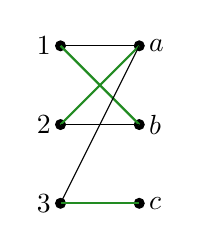
\begin{tikzpicture}
      \fill[black] (0, 0) circle (2pt) node[left] {$1$};
      \fill[black] (0, -1) circle (2pt) node[left] {$2$};
      \fill[black] (0, -2) circle (2pt) node[left] {$3$};
      \fill[black] (1, 0) circle (2pt) node[right] {$a$};
      \fill[black] (1, -1) circle (2pt) node[right] {$b$};
      \fill[black] (1, -2) circle (2pt) node[right] {$c$};
      \draw (0, 0) -- (1, 0);
      \draw[ForestGreen, thick] (0, 0) -- (1, -1);
      \draw[ForestGreen, thick] (0, -1) -- (1, 0);
      \draw (0, -1) -- (1, -1);
      \draw (0, -2) -- (1, 0);
      \draw[ForestGreen, thick] (0, -2) -- (1, -2);
    \end{tikzpicture}
    \caption{Another perfect matching in $G$.}
    \label{subfig:pm2}
  \end{subfigure}
  \caption{An example of matchings and the Tutte matrix.}
  \label{fig:example}
\end{figure}

\begin{proposition} \label{prop:det}
  A bipartite graph $G$ has a perfect matching if and only if $\det A_G \not \equiv 0$.
\end{proposition}

\begin{proof}
  Recall that
  $$ \det A_G = \sum_{\sigma: \text{ permutation of $n$}} \sign(\sigma) \prod_{i = 1}^n a_{i, \sigma(i)}. $$
  Note that $\sign(\sigma)$ is either $1$ or $-1$, and that $a_{i, \sigma(i)}$ is either $x_{i, \sigma(i)}$ or $0$. The main insight is that a permutation of $[n]$ corresponds to a potential perfect matching such that $(i, \sigma(i))$ is a potential edge in the matching. For each permutation $\sigma$ of $[n]$, $\prod_{i = 1}^n a_{i, \sigma(i)} = 0$ if one edge in the corresponding potential matching is missing, so $\prod_{i = 1}^n a_{i, \sigma(i)} \neq 0$ if and only if it corresponds to a perfect matching. Therefore, $\det A_G \not \equiv 0$ if and only if there exists one permutation $\sigma$ of $[n]$ which corresponds to a perfect matching.
\end{proof}

Note that $\det A_G$ is a polynomial on $n^2$ variables (one for each possible edge) of total degree $n$. Therefore, Proposition \ref{prop:det} gives Algorithm for testing whether a bipartite graph has a perfect matching. The total number of terms in $\det A_G$ is at most $n!$. However, we can use matrix multiplication algorithms to compute the determinant of a matrix in time that is polynomial in $n$.

\begin{algorithm}
  $A_G \leftarrow \text{the Tutte matrix of $G$}$ \\
  test whether $\det A_G \not\equiv 0$ \\
  \If{$\det A_G \not \equiv 0$}{
    output ``$G$ has a perfect matching''
  }
  \Else{
    output ``$G$ does not have a perfect matching''
  }
  \caption{An algorithm for testing whether a bipartite graph $G$ has a perfect matching.}
\end{algorithm}

\end{document}
